\documentclass[tikz,border=0.1cm]{standalone}
\usepackage{tikz}
\usetikzlibrary{shapes.geometric, arrows.meta}
% \usepackage{par_style}
\usetikzlibrary{positioning}

\newcommand{\stackednode}[5]{
  \begin{scope}
    % Background rectangles
    \node[draw=black, rounded corners, fill=green!10, minimum width=#3, minimum height=#4] 
      at ([shift={(0.4,0.2)}]#2) {};
    \node[draw=black,rounded corners,  fill=green!10, minimum width=#3, minimum height=#4] 
      at ([shift={(0.25,0.1)}]#2) {};

    % Foreground named node with text
    \node (#1) [draw=black,rounded corners,  fill=green!10, text width=#3, align=center, line width=1pt] 
      at (#2) {#5};
  \end{scope}
}


\tikzstyle{startstop} = [rectangle, rounded corners, minimum width=2.7cm, minimum height=1cm,
                         text centered, draw=black, fill=gray!20, line width=1pt ]
\tikzstyle{cat}       = [rectangle, rounded corners, minimum width=2.7cm, minimum height=1cm,
                         text centered, draw=black, fill=white!10, line width=1pt ]
\tikzstyle{arrow}     = [thick,->,>=stealth]
\tikzstyle{process} = [rectangle, rounded corners,minimum width=4.3cm, minimum height=1cm, text centered, draw=black, fill=blue!10, line width=1pt ]

\begin{document}
\begin{tikzpicture}

% Top node
\node (start) at (0,0) [startstop] {Input Data};

% Three submodules
\node (processing)   at (-5,-3) [cat] {Processing};
\node (analysis)      at (0,-3)  [cat] {Analysis};
\node (vis) at (5.5,-3)  [cat] {Visualization};

% Central vertical arrow
\draw [arrow] (start.south) -- (analysis.north);

% L-shaped arrows branching left and right
\draw [arrow, rounded corners] (start.south) -- ++(0,-1) -- (-5,-1.5) -- (processing.north);
\draw [arrow, rounded corners] (start.south) -- ++(0,-1) -- ( 5.5,-1.5) -- (vis.north);


%% ANALYSIS
\stackednode{chunk}{0,-5}{4.3cm}{1cm}{Read Data\\ in Chunks}
\draw[->] (analysis) -- (chunk);
\stackednode{parallelproc}{0,-7}{4.3cm}{1cm}{Parallel Processing\\ of Chunks}
\draw[->] (chunk) -- (parallelproc);
\stackednode{tempgeotiff}{0,-9}{4.3cm}{1cm}{Write to\\Temp GeoTIFFs}
\draw[->] (parallelproc) -- (tempgeotiff);
\node (mosaic) at (0,-11) [process] {Mosaic All output Chunks};
\node (save)at (0,-13)  [startstop,text width=4.3cm, align=center] {Save Final Raster Output(s)\\(.bin, .tif)};
\draw [arrow] (parallelproc) -- (tempgeotiff);
\draw [arrow] (tempgeotiff) -- (mosaic);
\draw [arrow] (mosaic) -- (save);

%% VISUALIZATION
\node (readplot) at (5.5,-5) [process] {Read Data};
\node (genplot) at (5.5,-7) [process,text width=4.3cm, align=center] {Generate Quick-looks\\or Plots (.png)};
\node (saveplot) at (5.5,-9) [startstop,text width=4.3cm, align=center]{Save output (.png)};
\draw [arrow] (vis) -- (readplot);
\draw [arrow] (readplot) -- (genplot);
\draw [arrow] (genplot) -- (saveplot);



%% Processing
\node (readplot) at (-5,-5) [process] {Import Data};
\node (genplot) at (-5,-7) [process,text width=4.3cm, align=center] {Generate standard \ PolSAR matrices};
\node (saveplot) at (-5,-9) [startstop,text width=4.3cm, align=center]{Save output (.tif/.bin)};
\draw [arrow] (processing) -- (readplot);
\draw [arrow] (readplot) -- (genplot);
\draw [arrow] (genplot) -- (saveplot);


% Legend
\node[draw=white, align=left, fill=white, anchor=north east] at (-3,-10.5) {
  \textbf{Legend:} \\

    \tikz[baseline]{
    \node[inner sep=0pt] (legenditem) at (0,0) {
        \begin{tikzpicture}
        \node[draw=black, rounded corners, fill=gray!20, minimum width=.6cm, minimum height=.4cm] {};
        \end{tikzpicture}
    };
    \node[anchor=west] at (legenditem.east) {~Input/Output Node};
    } \\

    \tikz[baseline]{
    \node[inner sep=0pt] (legenditem) at (0,0) {
        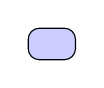
\begin{tikzpicture}
        \node[draw=black,  rounded corners, fill=blue!20, minimum width=.6cm, minimum height=.4cm] {};
        \end{tikzpicture}
    };
    \node[anchor=west] at (legenditem.east) {~Processing Step};
    } \\ 
    \tikz[baseline]{
  \node[inner sep=0pt] (legenditem) at (0,0) {
    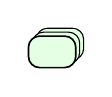
\begin{tikzpicture}
      % Back layer
      \node[draw=black, rounded corners,  fill=green!10, minimum width=0.6cm, minimum height=0.4cm] 
        at (0.1,0.1) {};
      % Mid layer
      \node[draw=black,rounded corners,  fill=green!10, minimum width=0.6cm, minimum height=0.4cm] 
        at (0.05,0.05) {};
      % Front layer
      \node[draw=black, rounded corners,  fill=green!10, line width=0.6pt, minimum width=0.6cm, minimum height=0.4cm] 
        at (0,0) {};
    \end{tikzpicture}
  };
  \node[anchor=west] at (legenditem.east) {Parallel Task};
    }\\

    \tikz[baseline]{
    \node[inner sep=0pt] (legenditem) at (0,0) {
        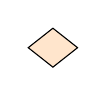
\begin{tikzpicture}
         \node[draw, diamond, aspect=2, inner sep=3pt, fill=orange!20, minimum height=.5cm] {};
        \end{tikzpicture}
    };
    \node[anchor=west] at (legenditem.east) {~Decision};
    } 
};




\end{tikzpicture}
\end{document}
